\begin{figure*}[ht]
    \centering
    \begin{subfigure}[t]{0.5\textwidth}
        \centering
        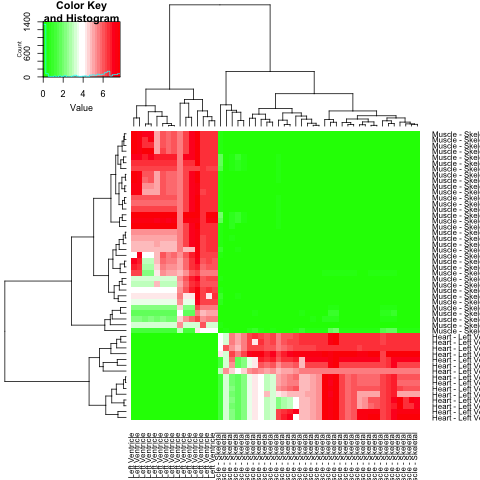
\includegraphics[height=3in]{../plots/heart_muscle_admixture_heatmap.png}
        \caption{Admixture proportions heatmap}
    \end{subfigure}%
    ~ 
    \begin{subfigure}[t]{0.5\textwidth}
        \centering
        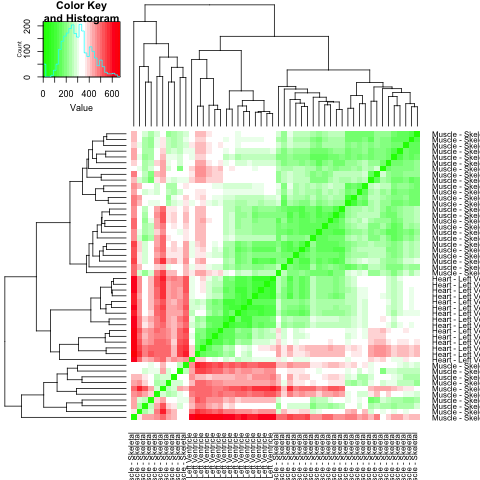
\includegraphics[height=3in]{../plots/heart_muscle_hierarchical_heatmap.png}
        \caption{Hierarchical cluster heatmap}
    \end{subfigure}
    \caption{Comparison of heatmap of the admixture proportions and heatmap due to hierarchical clustering on  a randomly drawn 50 samples from the pool of Muscle-Skeletal and Heart-Left Ventricle samples in GTEx Version 4 RNA-seq counts data. The distance method used euclidean and the linkage used was average linkage. Color scale provided in the figure. It seems that for admixture model heatmap, all the Muscle-skeletal and Heart Left-Ventricle samples cluster separately, while for the hierarchical model heatmap, they are mixed with each other. This suggests Admixture is better equipped at picking tissue separation than hierarchical clustering.}
\end{figure*}

\begin{figure*}[ht]
	\raggedleft
	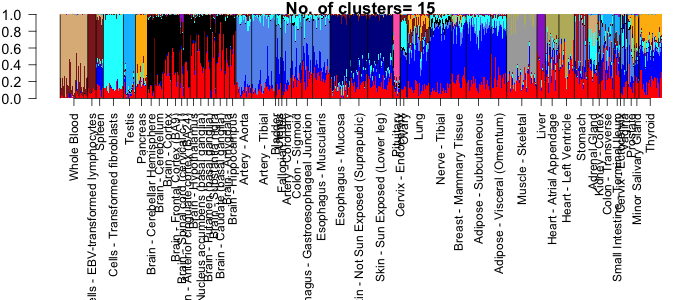
\includegraphics[height=3in, width=6.5in]{../plots/whole_tissue_structure_15.png}
        \caption{Structure plot of the admixture proportions (with 15 topics/clusters) for all the tissue samples in GTEX Version 4 data based on $5000$ genes with the highest mean expression. Some of the tissues form very distinct clusters, for instance Whole Blood, Pancreas, Skin, Arteries etc while there is a lot of similarity in cluster patterns between Muscle Skeletal and Heart Left Ventricle, or among the different sub-tissues of the Brain.}
\end{figure*}

\begin{figure*}[ht]
	\raggedleft
	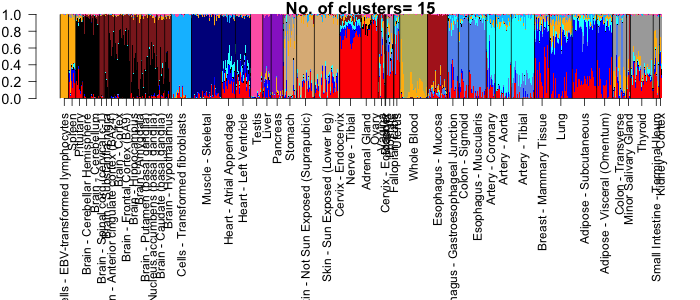
\includegraphics[height=3in, width=6.5in]{../plots/whole_tissue_structure_15_thinned.png}
        \caption{Structure plot of the admixture proportions (with 15 topics/clusters) for all the tissue samples in GTEX Version 4 data based on 16407 cis genes from the eQTL study conducted by the GTEx Consortium. Many of the patterns in this Structure plot are retained from the Structure plot based on the $5000$ genes with highest mean expression. }
\end{figure*}

\begin{figure*}[ht]
\centering
  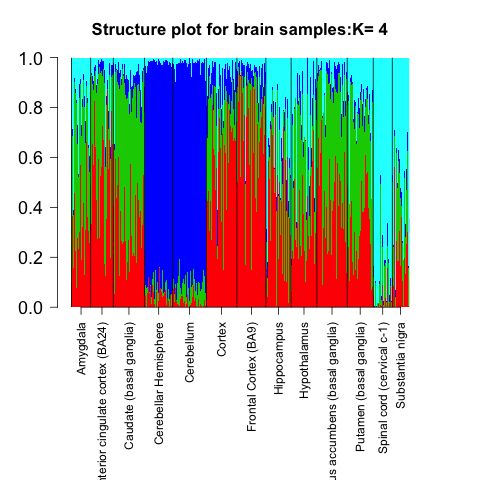
\includegraphics[height=3in, width=4.5in]{../plots/brain_structure_plot.png}
    \caption{Structure plot of the admixture proportions (with 4 clusters) for the brain tissue samples drawn from GTEX Version 4 data. Quite clearly, brain cerebellum and cerebellar hemisphere seem to be dominated by the blue cluster while the Spinal cord and Substantia nigra by the cyan cluster. Prior marker based approaches have verified (?) that $80 \%$ of cells in brain cerebellum correspond to neurons. So, the blue cluster seems to be driven by the neuron cell type. This fact is further attested by the gene annotations of the top genes driving the blue cluster (Subsection 3.3).}
\end{figure*}

 \begin{figure*}[ht]
    \raggedright
     \begin{subfigure}[t]{0.25\textwidth}
        \raggedleft
        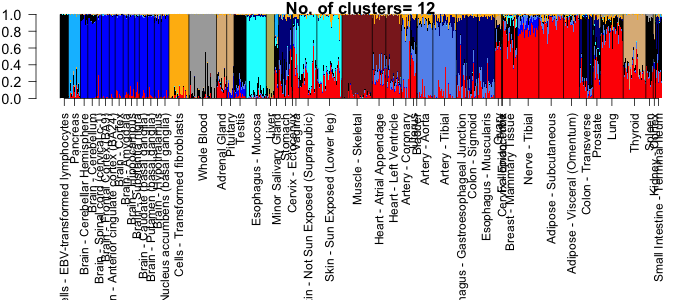
\includegraphics[height=2.7in]{../plots/gtex_thinned_clus_12_version_1.png}
        \caption{$p_{thin}=0.001$}
    \end{subfigure}    \\
    \begin{subfigure}[t]{0.25\textwidth}
        \raggedleft
        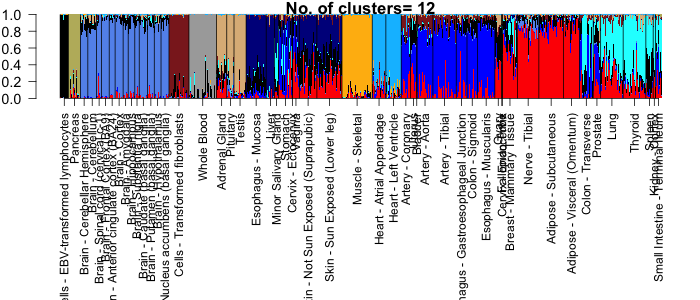
\includegraphics[height=2.7in]{../plots/gtex_thinned_clus_12_version_2.png}
        \caption{$p_{thin}=0.0001$}
    \end{subfigure}   
    \caption{Structure plot of all tissue samples in GTEx version 4 data for K=12 under different values of the thinning parameter $p_{thin}$. The three values of the thinning parameter chosen are $0.01$, $0.001$ and $0.0001$. It seems the results are pretty robust, though some of the cluster patterns seem to change. For instance, Muscle Skeletal and Heart tissue samples separate out at $p_{thin}=0.0001$ but cluster together at $p_{thin}=0.001$ for the same number of topics.}
    \end{figure*}
    
    

\begin{figure*}[ht]
    \centering
    \begin{subfigure}[t]{0.5\textwidth}
        \centering
        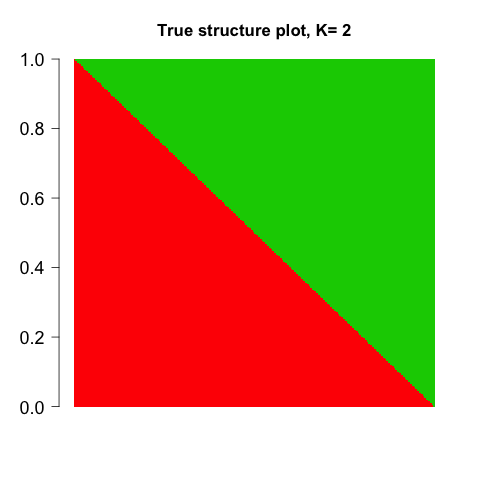
\includegraphics[height=3in]{../plots/true_structure_setup_1.png}
        \caption{Set up 1 (true structure)}
    \end{subfigure}%
    ~ 
    \begin{subfigure}[t]{0.5\textwidth}
        \centering
        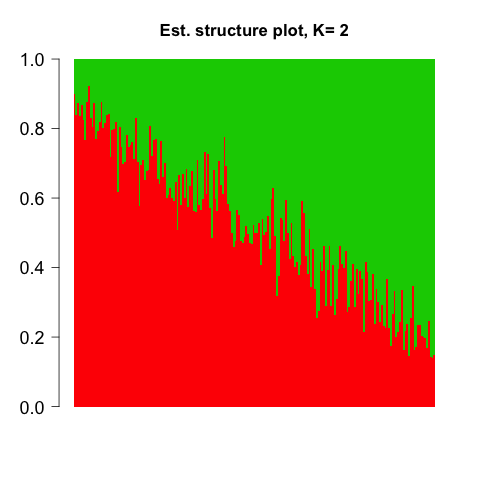
\includegraphics[height=3in]{../plots/est_structure_setup_1.png}
        \caption{Set up 1 (est. structure)}
    \end{subfigure}   \\
    
    \begin{subfigure}[t]{0.5\textwidth}
        \centering
        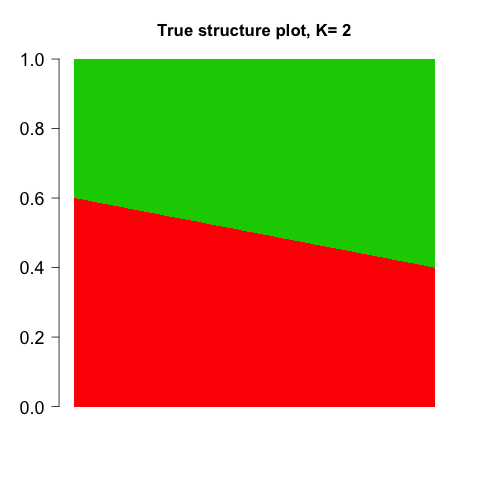
\includegraphics[height=3in]{../plots/true_structure_setup_2.png}
        \caption{Set up 2 (true structure)}
    \end{subfigure}%
    ~ 
    \begin{subfigure}[t]{0.5\textwidth}
        \centering
        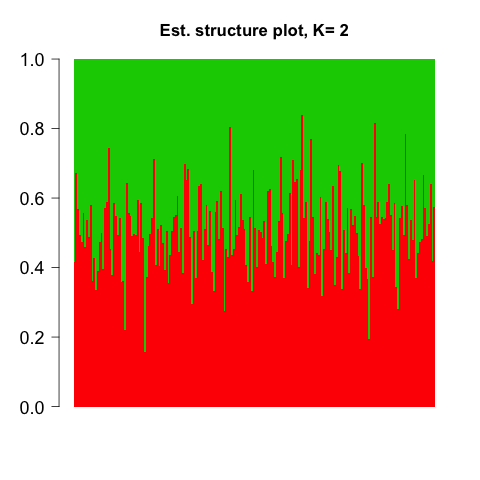
\includegraphics[height=3in]{../plots/est_structure_setup_2.png}
        \caption{Set up 2 (est. structure)}
    \end{subfigure} 
    \caption{A case study to check for the performance of the admixture model under two set ups, one where the true admixture proportions vary a lot from 0 to 1 across samples for the two clusters and the other where the true admixture proportions vary mildly around $0.5$ (from $0.4$ to $0.6$) for the two clusters. It is found that the admixture model is able to distinguish the clusters better in the first set up compared to the second. Even from gene annotations point of view, it is found that the admixture model is able to extract the truly significantly enriched genes for the clusters in the first set up but fails to do so in the second set up.}
 \end{figure*}
 
 
 \begin{figure*}[ht]
    \centering
    \begin{subfigure}[t]{0.5\textwidth}
        \centering
        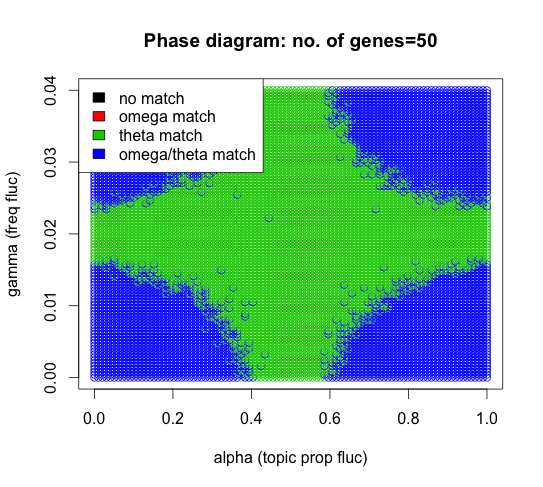
\includegraphics[height=3in]{../plots/phase_plot_50.png}
        \caption{G=50}
    \end{subfigure}%
  ~ 
    \begin{subfigure}[t]{0.5\textwidth}
        \centering
        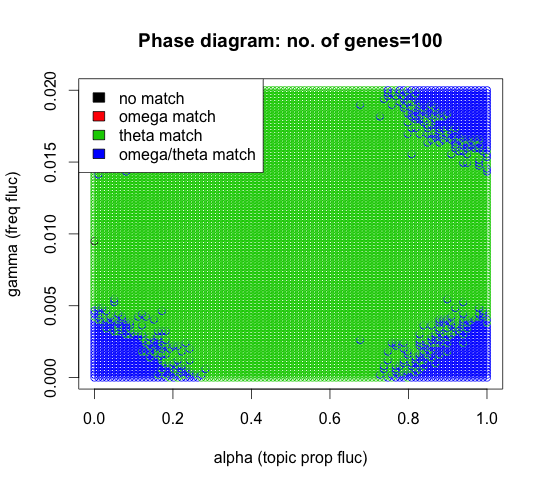
\includegraphics[height=3in]{../plots/phase_plot_100.png}
        \caption{G=100}
    \end{subfigure}   
      ~ 
    \begin{subfigure}[t]{0.5\textwidth}
        \centering
        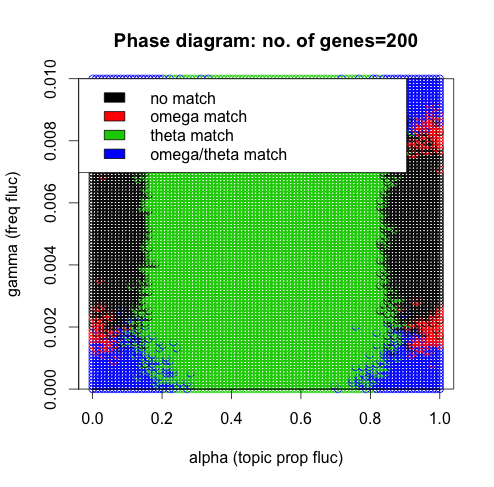
\includegraphics[height=3in]{../plots/phase_plot_200.png}
        \caption{G=200}
    \end{subfigure}   
    \caption{Phase diagram analysis for number of samples $N=200$ and three choices of $G$, $50$, $100$ and $200$. Note that as $G$ increases, the gene expression signal and the distance between the relative gene expression between the two clusters decreases. As a result, the performance of the admixture model deteriorates. Also, for a broad part of the phase space, though the admixture model does not manage to determine the admixture proportions well enough (\textit{omega match} does not hold) but it is able to extract the actually important genes driving the clusters (\textit{theta match} holds).}
    \end{figure*}
    
 
 \begin{figure*}[ht]
    \centering
    \begin{subfigure}[t]{0.5\textwidth}
        \centering
        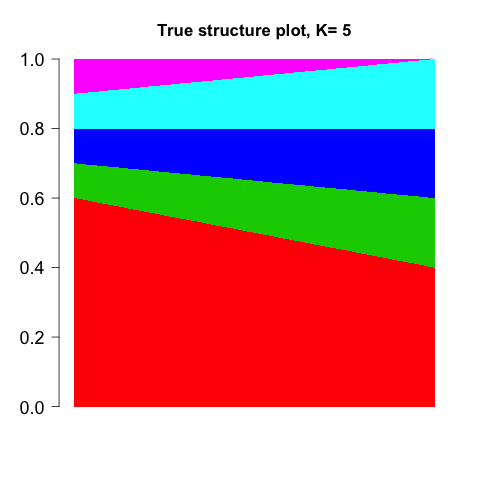
\includegraphics[height=3in]{../plots/true_structure_setup_3.png}
        \caption{Set up 3 (true structure)}
    \end{subfigure}%
    ~ 
    \begin{subfigure}[t]{0.5\textwidth}
        \centering
        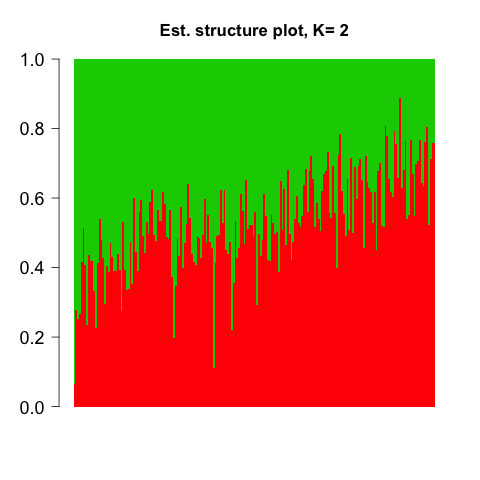
\includegraphics[height=3in]{../plots/est_structure_setup_3.png}
        \caption{Set up 3 (est. structure)}
    \end{subfigure}
    \caption{The true structure plot for a simulation set up with $N=1000$ samples nd $G=500$ genes with $K=5$ clusters where the admixture proportions are given in (a). Counts data were generated under this true simulation set up. Then admixture model was fitted for $K=2$ and the estimated Structure plot from the model fit is shown in (b).}
\end{figure*}


 \begin{figure*}[ht]
    \raggedright
     \begin{subfigure}[t]{0.3\textwidth}
        \raggedleft
        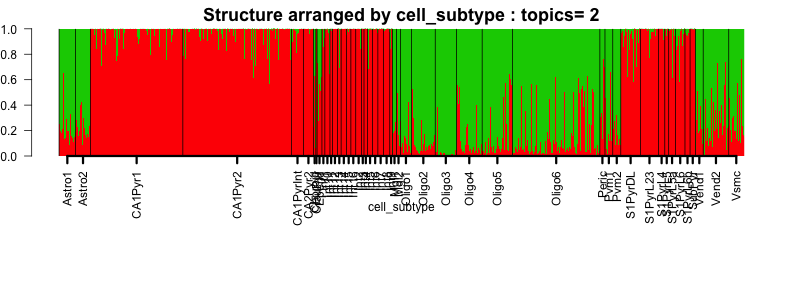
\includegraphics[height=2.5in]{../plots/Zeisel/clus_2/struct_clus_2_cell_subtype.png}
        \raggedright 
        \vspace{-0.5in} \qquad  \qquad  \caption{$k=2$}
    \end{subfigure}    \\
    \begin{subfigure}[t]{0.5\textwidth}
        \raggedleft
        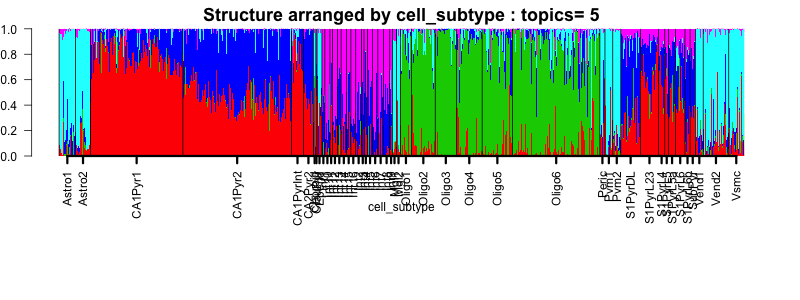
\includegraphics[height=2.5in]{../plots/Zeisel/clus_5/struct_clus_5_cell_subtype.png}
        \raggedright
        \vspace{-0.5in}  \qquad  \qquad \caption{$k=5$}
    \end{subfigure}    \\
    \begin{subfigure}[t]{0.5\textwidth}
        \raggedleft
        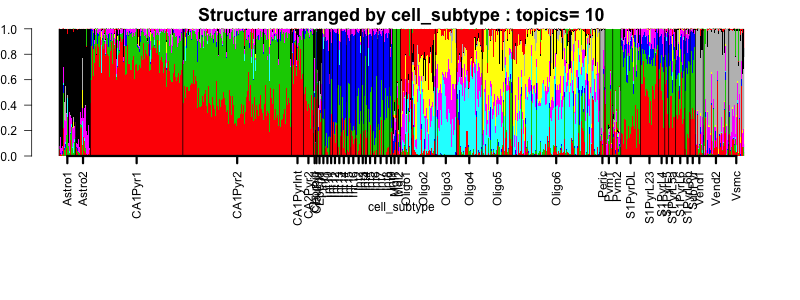
\includegraphics[height=2.5in]{../plots/Zeisel/clus_10/struct_clus_10_cell_subtype.png}
        \raggedright
        \vspace{-0.5in}  \qquad \qquad \caption{   $k=10$}
    \end{subfigure}    
    \caption{Structure plot of all  samples in Zeisel et al data \cite{Zeisel2015} arranged by the cell subtype labels that were determined by the authors using their BackSpin algorithm and subsequent marker gene annotations. Here we present the Structure plots for number of topics $k=2,5,10$. }
    \end{figure*}

